\subsection{Applying Transformers}
\label{sec:xformers}

We modify the \RVM semi-space copying collector~\cite{BCM:04,
Cheney:70}\index{semi-space copying collector} to update changed objects as
part of a collection. The collector traverses the heap, copies reachable
objects, and creates additional empty copies for all updated live objects. After collection, \JV walks through these
updated objects, runs their object transformers, and sets their fields
appropriately. We first examine \RVM's semi-space copying collector and the
tricolor abstraction~\cite{Dijkstra78, JL:96}\index{tricolor abstraction}
it maintains, and then present \JV's modifications.

In the tricolor abstraction, the \GC maintains colors for each object as it
performs a full-heap traversal to compute the transitive closure of
reachable objects. Objects have one of three colors: white objects are yet
to be visited; black objects have been visited and their immediate children
have been visited has well; grey objects have been visited but their
children might not have been visited. In this abstraction, collectors
maintain the invariant that no black object can point to
a white object. At the end of the traversal, there are no grey objects.
Objects that are unreachable are white and are freed by the
collector. Reachable objects are black and survive the collection.

\BCode[p]{0.75}
\begin{lstlisting}[frame=single, escapeinside={(*}{*)}]
function GC(roots):
   Q := empty
   for r in roots:
       r.color = GREY
       Q.add(r)
   while Q not empty:
       object = Q.pop()
       scanObject(object)

// precondition: object is GREY
function scanObject(object):(*\label{line:scan}*)
    for field in object:
        object.field = moveObject(object.field)
    object.color = BLACK

// precondition: object is either a forwarding
// pointer or a WHITE object. Either way,
// object resides in from space.
function moveObject(object):
    if object is real:
        copy = copyObject(object)
        copy.color = GREY
        Q.add(copy)
        object.FP = copy
        return copy
    if object is a forwarding pointer:
        return object.FP

// precondition: object is WHITE
function copyObject(object):
    copy = malloc() # in to space
    memcopy(copy, object)
    return copy
\end{lstlisting}
\ECode{Semi-space copying collector pseudo-code\label{fig:gc-code}}


The semi-space collector maintains the tricolor abstraction as follows. The
heap is divided into two spaces --- the currently active heap with all
objects, called the {\em from-space}, and an empty heap called {\em
to-space}. During the traversal, the collector copies reachable objects
from from-space to to-space and leaves unreachable ones in from-space. At
the end of collection, the entire from-space is reclaimed. Initially, all
objects in from-space are colored white. The traversal begins at {\em
roots}. The roots include statics, stack-allocated local variables, and
references in registers. The compiler generates a {\em stack map} at every
\VM safe point (a superset of \USD safe points).  The stack map enumerates
all register and local variables on the stack that reference heap objects.
The roots are not objects themselves, but are references to objects. The
roots reside outside the heap and are not copied. For the purposes of the
tricolor abstraction, the roots are initially colored gray.

The copying
collector walks through the list of grey objects and {\em scans} them (see
line~\ref{line:scan} in Figure~\ref{fig:gc-code}). Scanning an object
involves going through all reference fields of that object, moving the
referred objects over to to-space, and setting the field to the address
newly moved to. When moving an object, the collector leaves behind a {\em
forwarding pointer} in its place that points to the new location. This pointer
ensures that an object is moved only once and the forwarding pointer gives the
to-space address 
of the object. Later, if the collector encounters a
forwarding pointer when processing a reference, it sets the reference to
the value of the forwarding pointer.
Moving an object to to-space turns it
grey, while scanning an object makes it black. The fields of black objects
point to other objects in to-space, which are either grey or black.  The
fields of grey objects point to white objects (or forwarding pointers),
which are in from-space.
% \todo{You asked me to change the previous sentence to ``white objects or
% black objects that contain forwarding pointers''. Not sure if that is
% correct}
The traversal ends when there are no more grey
objects.

% We modify the \RVM semi-space copying collector \cite{BCM:04, Cheney:70} to update
% changed objects as part of a collection. The collector transforms old
% objects of an updated classes to conform to their new class signature and
% point to their new \acf{TIB}.  A semi-space copying collector normally
% works by traversing the pointer graph in the old heap (called
% \emph{from-space}) starting at the \emph{roots} and performing a transitive
% closure over the object graph, copying all objects it encounters to a new
% heap (called \emph{to-space}).  The roots include statics, stack-allocated
% local variables, and references in registers.  The compiler generates a
% \emph{stack map} at every VM safe point (a superset of DSU safe points).
% The stack map enumerates all register and local variables on the stack that
% reference heap objects.  When the collector first encounters an object, it
% copies it to to-space and then overwrites its header with a forwarding
% pointer to the new copy.  If the collector encounters a forwarded object
% later via another reference, it uses the forwarding pointer to redirect the
% reference to the new object. Forwarding pointers help the collector
% maintain the tricolor garbage collector invariant \cite{Dijkstra78, JL:96}
% and ensure each live object is copied exactly once, and all references to
% such an object point to the copy in to-space.

\BCode[p]{0.75}
\begin{lstlisting}[frame=single]
function moveObject(object):
    if object is real:
        copy = copyObject(object)
        copy.color = GREY
        Q.add(copy)
        if object.type.newVersion != null:
           newCopy = malloc()
           add newCopy to update log
           newCopy.type = object.type.newVersion
           // newCopy is currently empty
           object.FP = newCopy
           return newCopy
        else:
           object.FP = copy
           return copy
    if object is a forwarding pointer:
        return object.FP
\end{lstlisting}
\ECode{\JV's modification to \RVM's semi-space copying collector\label{fig:jvolve-gc-code}}


\begin{figure}[p]
\centering
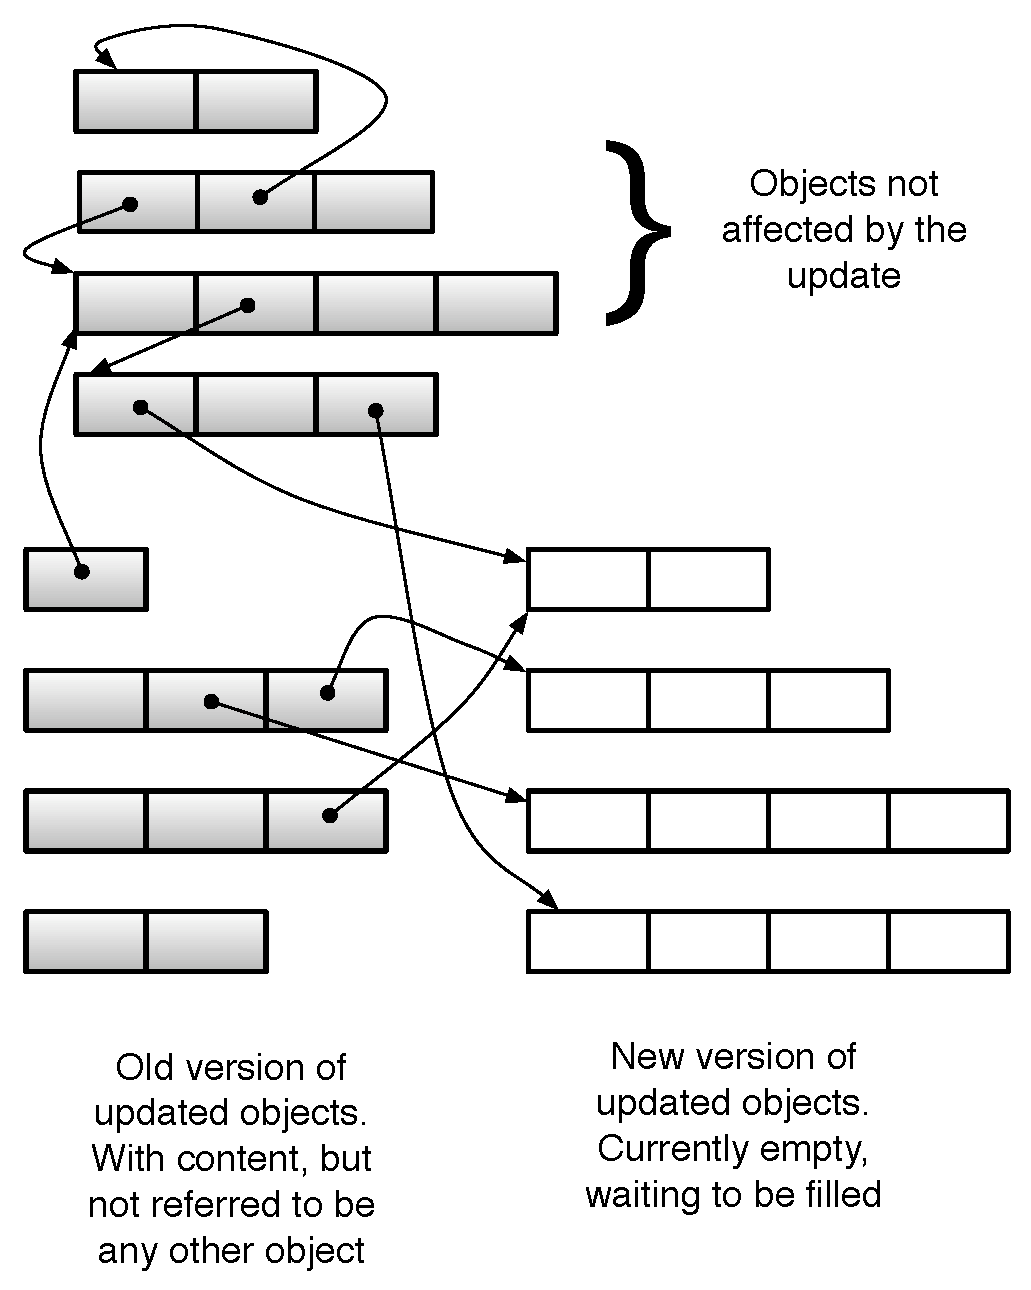
\includegraphics[scale=0.35]{100-images/to-space-after-gc}
\caption{A view of the \emph{to} semi-space immediately after garbage
collection\label{fig:to-space-after-gc}}
\end{figure}

\JV's modified collector works in much the same way as the regular
semi-space collector just described. As shown in
Figure~\ref{fig:jvolve-gc-code}, it differs in how it handles objects whose
class signature has changed.  In this case, it allocates a copy of the old
object \emph{and} an \emph{empty} new object according to the new class
definition, which may
have a different size compared to the old one. The collector initializes
the new object to point to the \acf{TIB}\iTIB of the new type, and installs the
forwarding pointer in from-space to this new version.  Next, the collector
stores a pair of pointers in its \emph{update log}, one to the copy of the
old object and one to the new object.  The collector continues scanning the
old copy. The key fact to note is that because forwarding pointers point to
the empty new copy of the object, references to updated types all point to
these empty objects.  Figure~\ref{fig:to-space-after-gc} illustrates this
situation. The old version of updated objects are filled with content while
references point to empty new versions of these objects.

After the collection completes, \JV adds another phase. It
first executes transformers for all
classes and then for all objects. 
%MWH: either order does not work equally well; both are wrong, really, but
%the current order is less likely to be wrong. See long e-mail exchange
%with %Suriya a while back.  We don't really handle this case correctly
%right now, so better to say little.
\JV goes through the update log and invokes the object transformer,
passing the old and new object pair as arguments. Recall from
Section~\ref{subsec:transformers} that the \JO functions receive an object
of the old version and an object of the new version as parameters. These
parameters come from the update log, with the old object filled with
content and the new object empty waiting to be filled by the transformer
function. Once \JV processes all object pairs, the log is deleted, making
the  duplicate old versions unreachable.
As Figure~\ref{fig:to-space-after-gc} shows, old version objects are
unreachable as no references point to them, and the next garbage collection
cycle will free them. While we did not do so in our implementation, we
could put these objects in a special space and reclaim the space
immediately after the update. We now look at two simple updates to
illustrate how \JV applies object transformers.

\begin{figure}[t]
\centering
\includegraphics[scale=0.7]{100-images/gcupdate}
\caption{Running object transformers following garbage collection}
\label{fig:gc-example}
\end{figure}

\paragraph{Example 1.} Figure~\ref{fig:gc-example} illustrates a part of
the heap at the end of the GC phase while applying the update from
Figure~\ref{fig:jes-transformer-code} (forwarding pointers are not shown).
On the
left is a depiction of part of the heap prior to the update.  It shows a
\User object whose fields point to various other elided objects.
After the copying phase, all of the old reachable objects are duplicated in
to-space.  The transformation log points to the new version of \User
(which is initially empty) and the duplicate of the old version, both of
which are in to-space.  The transformer function can safely copy fields of
the \FROM object. The figure shows that after running the transformer
function, the new version's {\tt username} field points to the same object
as before, and the new version's {\tt forwardAddresses} field points to a
new array of new {\tt EmailAddress} objects.
The {\tt EmailAddress} constructor called from within the
transformer function initialized these objects by referring to the old
e-mail {\tt String} values and assigning fields to point to substrings of
the given {\tt String}.

\begin{figure}[t]
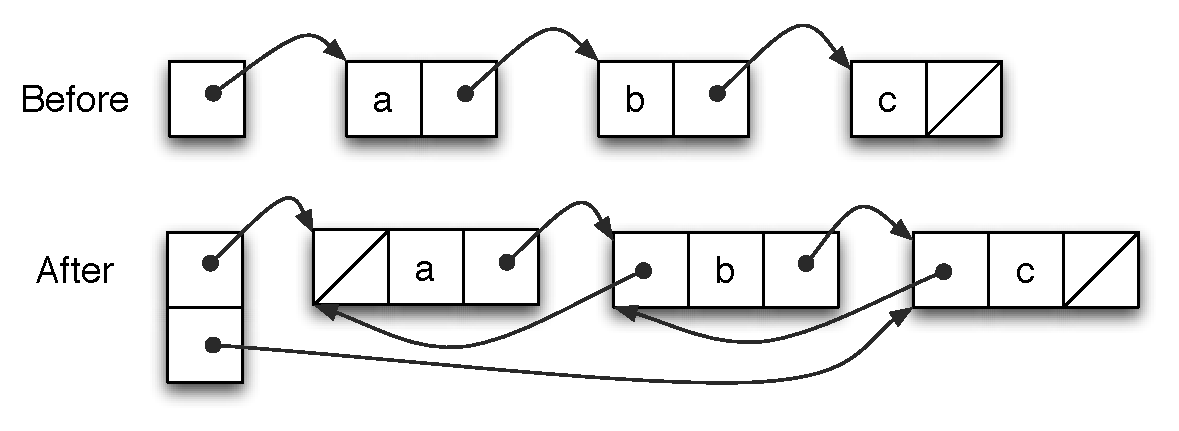
\includegraphics[scale=0.7]{100-images/linked-lists-without-gc}
\hangcaption{A look at the structure of an example linked list before and after the update
\label{fig:before-after-singly-doubly}}
\VspaceFixForHangcaption
\end{figure}

\begin{figure}[p]
\lstset{frame=single}
\begin{center}
\begin{tabular}{@{}c@{\hspace{0.07\textwidth}}c@{}}
\begin{minipage}{0.42\textwidth}
\begin{lstlisting}[title={Old version code}]
public class LinkedList {
  class Node {
    Node next;
    int data;
  }
  private Node head;
}
\end{lstlisting}
\end{minipage} &
\begin{minipage}{0.42\textwidth}
\begin{lstlisting}[title={New version code}]
public class LinkedList {
  class Node {
    Node prev;
    Node next;
    int data;
  }
  private Node head;
  private Node tail;
}
\end{lstlisting}
\end{minipage}
\end{tabular} \\[2ex]
\begin{minipage}{0.9\textwidth}
\begin{lstlisting}[frame=single,title={Stub classes for the old version}]
public class r0_LinkedList {
  public LinkedList.Node head;
  public class Node {
    public LinkedList.Node next;
    public int data;
  }
}
\end{lstlisting}
\end{minipage} \\[2ex]
\begin{minipage}{0.9\textwidth}
\begin{lstlisting}[frame=single,title={Default \UPT-generated transformer}]
public class JvolveTransformers {
  public static void jvolveObject(
      LinkedList.Node to, r0_LinkedList.Node from) {
    to.prev = null; // no such field in from
    to.next = from.next;
    to.data = from.data;
  }
  public static void jvolveClass(LinkedList.Node unused) {}
  public static void jvolveObject(
      LinkedList to, r0_LinkedList from) {
    to.head = from.head;
    to.tail = null; // no such field in from
  }
  public static void jvolveClass(LinkedList unused) {}
}
\end{lstlisting}
\end{minipage}
\end{center} 
\vspace*{-2ex}
% 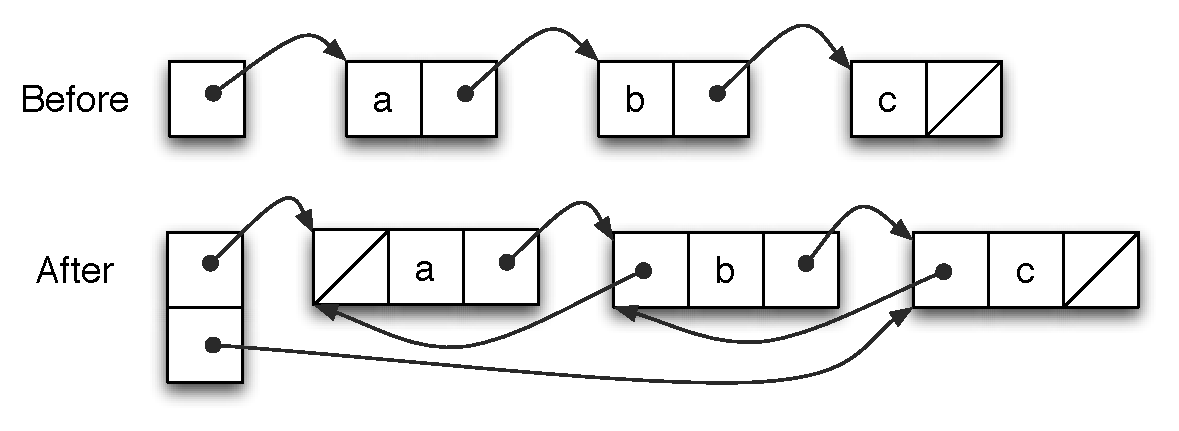
\includegraphics[scale=0.7]{100-images/linked-lists-without-gc}
\caption{An update that goes from a singly-linked to a doubly-linked list
\label{fig:singly-doubly}}
\lstset{frame=none}
\end{figure}


\paragraph{Example 2.}
We explore our object transformation\index{object transformer} model
by looking at another example.
Figure~\ref{fig:before-after-singly-doubly} shows an example linked list
before and after the update. In this example, a singly-linked list in the
old version becomes a doubly-linked list in the new.
Figure~\ref{fig:singly-doubly} shows the code for the old and new versions,
and stub classes and default transformers generated by the \acf{UPT}.
The update involves two classes with
signature changes: {\tt LinkedList} which adds a {\tt tail} field, and
{\tt Node} which adds a {\tt prev} field. The object transformers must
set these additional fields appropriately to create a doubly-linked list
out of a singly-linked one. The \JO functions generated by default will
correctly copy the {\tt data} and {\tt next} fields for each node in the
linked-list and correctly set {\tt head} to point to the start of the list.
We modify {\tt Node}'s transformer to set each node's {\tt next} node's
{\tt prev} field to point back to itself, i.e., {\tt from.next.prev =
from}.
Setting the {\tt tail} of the list to point to the last node is trickier.
We need some way to traverse the list to get to the end. At the time we
traverse the list, not all nodes might have been transformed. In order to
support this update, \JV provides a way for the programmer to request that
an object be transformed on-demand as the programmer traverses the list to
retrieve the {\tt tail} element of the list.  Section~\ref{sec:transformer-model}
explores this example in more detail and presents alternative object
transformation models.
